\documentclass[12pt,a4paper]{article}
\usepackage[utf8]{inputenc}
\usepackage{polski}
\usepackage{graphicx}
\usepackage{listings}
\author{Marcin TORGiren Fabrykowski}
\title{Analiza i przetwarzanie obrazu\\laboratorium 1}
\begin{document}
\lstset{language=Python}
\maketitle
\newpage
\section{Wstęp teoretyczny}
\subsection{Wyjaśnienie podstawowych pojęć}
\begin{description}
\item[Piksel] najmniejszy widzialny element obrazu na ekranie monitora. W~systemie RGB składa się z~trzech subpikseli o~kolorach: czerwonym (Red), zielonym (Green) oraz niebieskim (Blue). W~zależności od natężenia światła emitowanego przez pojedynczy subpiksel, wypadkowa barwa piksela zmienia się na zasadzie syntezy addytywnej. 
\item[Szum] zakłócenia na obrazie. Jest on skutkiem niedoskonałości technologii pobierającej obraz ze świata zewnętrznego (różnice w~czułości sąsiadujących elementów światłoczułych na matrycy). Jest on najbardziej widoczny gdy obraz powstał w~warunkach niedoboru światła. 
\item[Szum sztuczny] szum wygenerowany w~sposób pseudolosowy za pomocą komputera.
\item[Obraz ostry] przenosi dużą ilość informacji (często nadmiarowych), wszystkie detale obiektu są wyraźne i~łatwe do rozróżnienia.
\item[Obraz słaby] obraz zaszumiony, nieostry, rozmazany lub zmodyfikowany w~inny sposób utrudniający jego odczytanie. Często przenosi on zbyt mało informacji do poprawnej klasyfikacji.
\item[Wstępne przetwarzanie] operacje przeprowadzane na obrazie wejściowym, w~celu usunięcia zanieczyszczeń i~przygotowania do ekstrakcji cech.
\item[Projekcja (pozioma/pionowa)] zliczenie pikseli w~liniach lub kolumnach i~przedstawienie zależności jako wykresu (histogramu).
\item[Histogram] wykres słupkowy, przedstawiający zależność wartości cechy od jej ilości. W~analizie i~przetwarzaniu obrazów histogram oznacza w~szczególności wykres przedstawiający zależność wartości pikseli od ich ilości na obrazie. Oś pozioma zawiera rosnąco wartości pikseli od 0 do 255, natomiast oś pionowa - ilość wystąpień piksela o~danej wartości barwy. W~przypadku histogramu RGB każdy kanał rozpatrywany jest osobno.
\end{description}
\subsection{Przetwarzany obraz}
Obraz źródłowy znajduje się na rys.~\ref{fig:src}
\begin{figure}[h]

\includegraphics{tux}
\caption{Obraz źródłowy}
\label{fig:src}
\end{figure}
\newpage
\section{Analiza obrazu}
\subsection{Negatyw}
\subsubsection{Kod funkcji}
\begin{lstlisting}
    @image_loaded
    def negative(self):
        """Tworzy negatyw obrazu"""
        data = np.array(self.__image.getdata())
        data = 255 - data
        data = [tuple(x) for x in data]
        self.__image.putdata(data)
\end{lstlisting}
\subsection{Przetworzony obraz}
Przetworzony obraz jest widoczny na rys.~\ref{fig:neg}
\begin{figure}[h]

\includegraphics{negative}
\caption{Negatyw}
\label{fig:neg}
\end{figure}
\subsection{Odcienie szarości}
\subsubsection{Kod funkcji}
\begin{lstlisting}
def __grayscale1(self):
  """Konwersja do skali szarosci"""
  data = np.array(self.__image.getdata())
  data = [3 * (int(x.mean()),) for x in data]
  self.__image.putdata(data)

def __grayscale2(self):
  """konwersja do skali szarosci"""
  data = np.array(self.__image.getdata())
  data = [3 * (int(0.3 * x[0] + 0.59 * x[1] + 0.11 * x[2]),)
		for x in data]
  self.__image.putdata(data)
\end{lstlisting}
\subsubsection{Przetworzony obraz}
Przetworzony obraz jest widoczny na rys.~\ref{fig:gray}
\begin{figure}[h]
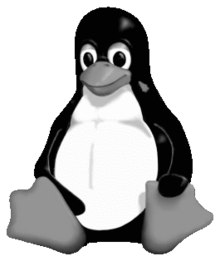
\includegraphics{grayscale1}
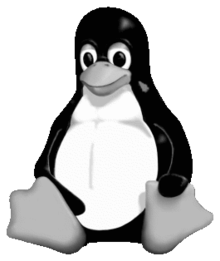
\includegraphics{grayscale2}
\caption{Obrazy w~skali szarości}
\label{fig:gray}
\end{figure}
\subsection{Normalizacja histogramu}
\subsubsection{Kod funkcji}
\begin{lstlisting}
    @image_loaded
    def normalize(self):
        data = np.array(self.__image.getdata())
        R = data[:, 0]
        G = data[:, 1]
        B = data[:, 2]
        R = (R - R.min()) * 255. / R.max()
        B = (B - B.min()) * 255. / B.max()
        B = (B - B.min()) * 255. / B.max()

        data[:, 0] = R
        data[:, 1] = G
        data[:, 2] = B

        data = [tuple(x) for x in data]
        self.__image.putdata(data)
\end{lstlisting}
\subsubsection{Przetworzony obraz}
Przetworzony obraz jest widoczny na rys.~\ref{fig:norm}
\begin{figure}[ht]
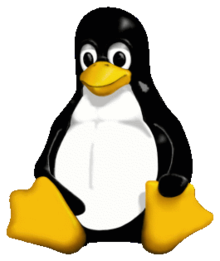
\includegraphics{normalize}
\caption{Obraz ze znormalizowanym histogramem}
\label{fig:norm}
\end{figure}
\section{Wnioski}
\begin{itemize}
\item Druga metoda konwersji do odcieni szarości daje lepszy wynik wizualny, ponieważ ludzkie oko jest bardziej czułe na kolor zielony, co zostało uwzględnione we wzorze.
W~przypadku pierwszej metody, wszystkie składowe mają taką samą wagę.
\item Wykonanie normalizacji histogramu pozwala na zwiększenie kontrastu obrazu.
\end{itemize}
\end{document}
